\documentclass[a4paper, 12pt]{article}
\usepackage[numbers,super,sort&compress,merge,mcite]{natbib}
\usepackage[latin1, utf8]{inputenc}
\usepackage[version=4]{mhchem} 
\usepackage[activeacute,english,spanish,es-tabla]{babel}
\usepackage{graphicx}
\usepackage{float}
\usepackage{times}
\usepackage{geometry}
\usepackage{fancyhdr}
\usepackage{lipsum}
\usepackage{setspace}
\usepackage{caption}
\usepackage{array,rotating,colortbl,longtable,tabulary,booktabs}
\usepackage[nottoc]{tocbibind}
\usepackage{wrapfig,subfigure}
\usepackage{tikz,pgfplots,pgfkeys}
\usepackage[bookmarks=true, hypertexnames=false, final, implicit, backref=false, linktocpage=false, colorlinks=true, allcolors=black, pdfpagelabels, plainpages=false, pdftex]{hyperref}
\pgfplotsset{compat=1.18}
\usetikzlibrary{er,shapes,arrows.meta,decorations.pathmorphing,backgrounds,positioning,fit,trees,calc,through,plotmarks}
\usetikzlibrary{calc} \tikzset{>=latex}

%%%%%%%%%%%%%%%%%%%%%%%%%%%%%%%%%%%%%%%%%%%%%%%%%%%%%%%%%%%%%%%%%%%%%%%%%%
%%%%%%%%%%%%%%%%%%%%%%%%%%%%%%%%%%%%%%%%%%%%%%%%%%%%%%%%%%%%%%%%%%%%%%%%%%
%%%%%%%%%%%%%%%%%%%%%% Configuración de la página %%%%%%%%%%%%%%%%%%%%%%%%
%%%%%%%%%%%%%%%%%%%%%%%%%%%%%%%%%%%%%%%%%%%%%%%%%%%%%%%%%%%%%%%%%%%%%%%%%%

\geometry{left=2.5cm, right=2.5cm, top=3cm, bottom=3cm}
\pagestyle{fancy}
\fancyhf{}
\fancyfoot[c]{\thepage}

%%%%%%%%%%%%%%%%%%%%%%%%%%%%%%%%%%%%%%%%%%%%%%%%%%%%%%%%%%%%%%%%%%%%%%%%%%%
%%%%%%%%%%%%%%%%%%% Configuración del interlineado %%%%%%%%%%%%%%%%%%%%%%%%
%%%%%%%%%%%%%%%%%%%%%%%%%%%%%%%%%%%%%%%%%%%%%%%%%%%%%%%%%%%%%%%%%%%%%%%%%%%

\onehalfspacing


\begin{document}

%%%%%%%%%%%%%%%%%%%%%%%%%%%%%%%%%%%%%%%%%%%%%%%%%%%%%%%%%%%%%%%%%%%%%%%%%%%
%%%%%%%%%%%%%%%%%%%%%%%%%%%%%%% Portada %%%%%%%%%%%%%%%%%%%%%%%%%%%%%%%%%%%
%%%%%%%%%%%%%%%%%%%%%%%%%%%%%%%%%%%%%%%%%%%%%%%%%%%%%%%%%%%%%%%%%%%%%%%%%%%

\begin{titlepage}
    \begin{center}
      
\includegraphics[width=4cm]{img/Sin título.png}\hfill
      
\includegraphics[width=3.5cm]{img/images.jpeg}\par
      \vspace{3cm}
      \textbf{Universidad Católica de Santa María}\\
      Facultad de Ciencias Farmacéuticas, Bioquímicas y Biotecnológicas\\
      Escuela Profesional de Ingeniería Biotecnológica\par
      \vfill
      \textbf{Informe de Prácticas Pre-Profesionales}\\
      Centro de Investigación en Ingeniería Molecular\par
      \vfill
      Quispe Ppacco, David Jonatán\\
      Arequipa, 2023
    \end{center}

\end{titlepage}

%%%%%%%%%%%%%%%%%%%%%%%%%%%%%%%%%%%%%%%%%%%%%%%%%%%%%%%%%%%%%%%%%%%%%%%%%%%
%%%%%%%%%%%%%%%%%%%%%%%%%%%%%%%% Índice %%%%%%%%%%%%%%%%%%%%%%%%%%%%%%%%%%%
%%%%%%%%%%%%%%%%%%%%%%%%%%%%%%%%%%%%%%%%%%%%%%%%%%%%%%%%%%%%%%%%%%%%%%%%%%%


\tableofcontents


\newpage

%%%%%%%%%%%%%%%%%%%%%%%%%%%%%%%%%%%%%%%%%%%%%%%%%%%%%%%%%%%%%%%%%%%%%%%%%%%
%%%%%%%%%%%%%%%%%%%%%%%%% Inicio del documento %%%%%%%%%%%%%%%%%%%%%%%%%%%%
%%%%%%%%%%%%%%%%%%%%%%%%%%%%%%%%%%%%%%%%%%%%%%%%%%%%%%%%%%%%%%%%%%%%%%%%%%%

\section{Introducción}

\begin{wrapfigure}{0}{0.3\textwidth}
     \vspace{-20pt}
        \begin{center}
            
\includegraphics[scale=0.46]{img/Sin título.jpeg}
        \end{center}
    \vspace{-20pt}
\end{wrapfigure}

Según la National Human Genome Research Institute, la bioinformática es  un vínculo que se encontró entre el campo de la biología y las ciencias informáticas con la capacidad de almacenar, analizar y recopilar datos, este campo está muy relacionado a la genética y genómica que se basa en la manipulación y análisis de datos para obtener como resultado el entendimiento de la fisiología celular cuando ocurre un cambio dentro de su entorno.


Comúnmente este campo nos enlaza con el análisis de secuencias y se aplica a los genes, ADN,  ARN o proteínas que resultan especialmente útiles para optimizar los experimentos en muchos ámbitos pueden hacer fricción con la divulgación científica. 

El Centro de Investigación en Ingeniería Molecular de la Universidad Católica de Santa María en la dirección del PhD Badhin Gómez Valdes presenta una de las mejores oportunidades para el inicio dentro de la comprensión estructural de la biología computacional a cargo de equipo multidisciplinario ha logrado muchos aportes en el campo de la comprensión de la fisiología celular a través de análisis informáticos.

El objetivo de este informe es presentar la estadía como practicante dentro de el Centro de Investigación en Ingeniería Molecular (CIIM), mostrando el avance de diversas actividades y conocimientos adquiridos hasta el momento de la presentación.


\section{Reseña de Actividades}
En este apartado mostramos el proceso, con aciertos y desaciertos encontrados en el desarrollo de las actividades realizadas en el CIIM. Cabe resaltar que las actividades realizadas en el centro de investigación postulan logros iniciales con proyección a que en los siguientes informes podamos ver logros realizados completados al igual que habilidades y destrezas desarrolladas:

    \subsection{Actividad 1: Inducción a la informática}

        \subsubsection {Objetivos}
            \begin{enumerate}
                \item Comprender la navegación en sistemas Linux
                \item Aplicar comandos usados en softwares sin interfaz gráfica (Gromacs)
            \end{enumerate}

        \subsubsection {Justificación}
        Para poder iniciar en el mundo de la bioinformática es básico conocer las características del software con el que contamos para poder hacer los cálculos o como coloquialmente se le llama las corridas de los diferentes métodos como lo es la dinámica molecular que lo explicaremos posteriormente. 

        Para este proceso es necesario comprender el sistema operativo "Ubuntu" que se usa en el CIIM, el sistema operativo que se usa es una "distro" de Linux que nos facilita la personalización de prioridades en cuanto a procesos ya que si usamos windows este sistema operativo al enfocarse en el confort del usuario genera procesos en segundo plano que no hacen mas que ralentizar los cálculos del análisis, pero allí viene la primera dificultad, el sistema Linux nos da mayor control de procesos al costo de sacrificar el confort.
    
        Linux es un sistema operativo que usa un tipo de lenguaje de programación incluido que es el lenguaje "Bash", es este lenguaje lo que hará la magia posteriormente para el análisis de datos ya que nos ofrece mayor automatización de procesos como lo es la comunicación directa con el programa de dinámica molecular Gromacs, que es un software que se encarga de  los cálculos de dinámica molecular.

        \subsubsection {Metodología}
        Para aprender este lenguaje se necesito de recurrir a los diferentes fuentes de información que nos puede ofrecer la nube, ya que en ella podemos encontrar los comandos más requeridos o básicos para realizar una buena ejecución en los terminales de Linux lo cual es importante para entender como funcionan los comandos para realizar una dinámica molecular o usar otras herramientas del software Gromacs, del que posteriormente se hablará.
        
        \subsubsection{Resultados esperados}
        Se pudo comprender la importancia de aplicar este lenguaje debido a su amplia versatilidad para interactuar tanto con la cpu como con los diversos softwares usados para la aplicación de el análisis de datos.

        Se espera no solo aprender un lenguaje de programación sino también aprender diversos debido a la alta demanda que tienen para optimizar sistemas de análisis de datos genómicos, en la actualidad contamos con múltiples herramientas de análisis de datos como lo es loa herramienta Pymol que trabaja principalmente con lenguaje Python3 también tenemos a FastQC que puede combinar Python3 con lenguaje R mientas y también tenemos a Gromacs cuya mayos afinidad se le ha visto con el lenguaje Bash ya que es más intuitivo y fácil de aprender. 

        La optimización constante de cada uno de los softwares que usamos para el análisis de datos nos impulsará a tener resultados más instantáneos y poder comprender los diversos mecanismos que se encuentran en el organismo a través de softwares informáticos, es por ello que presenta una alta importancia de que una persona que desee iniciar en el campo de la bioinformática tenga conocimiento de como es que las computadoras gestionan los datos ingresados. 

        \subsubsection{Evidencias}
        Se adjuntan el desarrollo de aprendizaje del lenguaje de programación: \ref{Fig:BashScript}

        \begin{figure}[H]
            \centering
            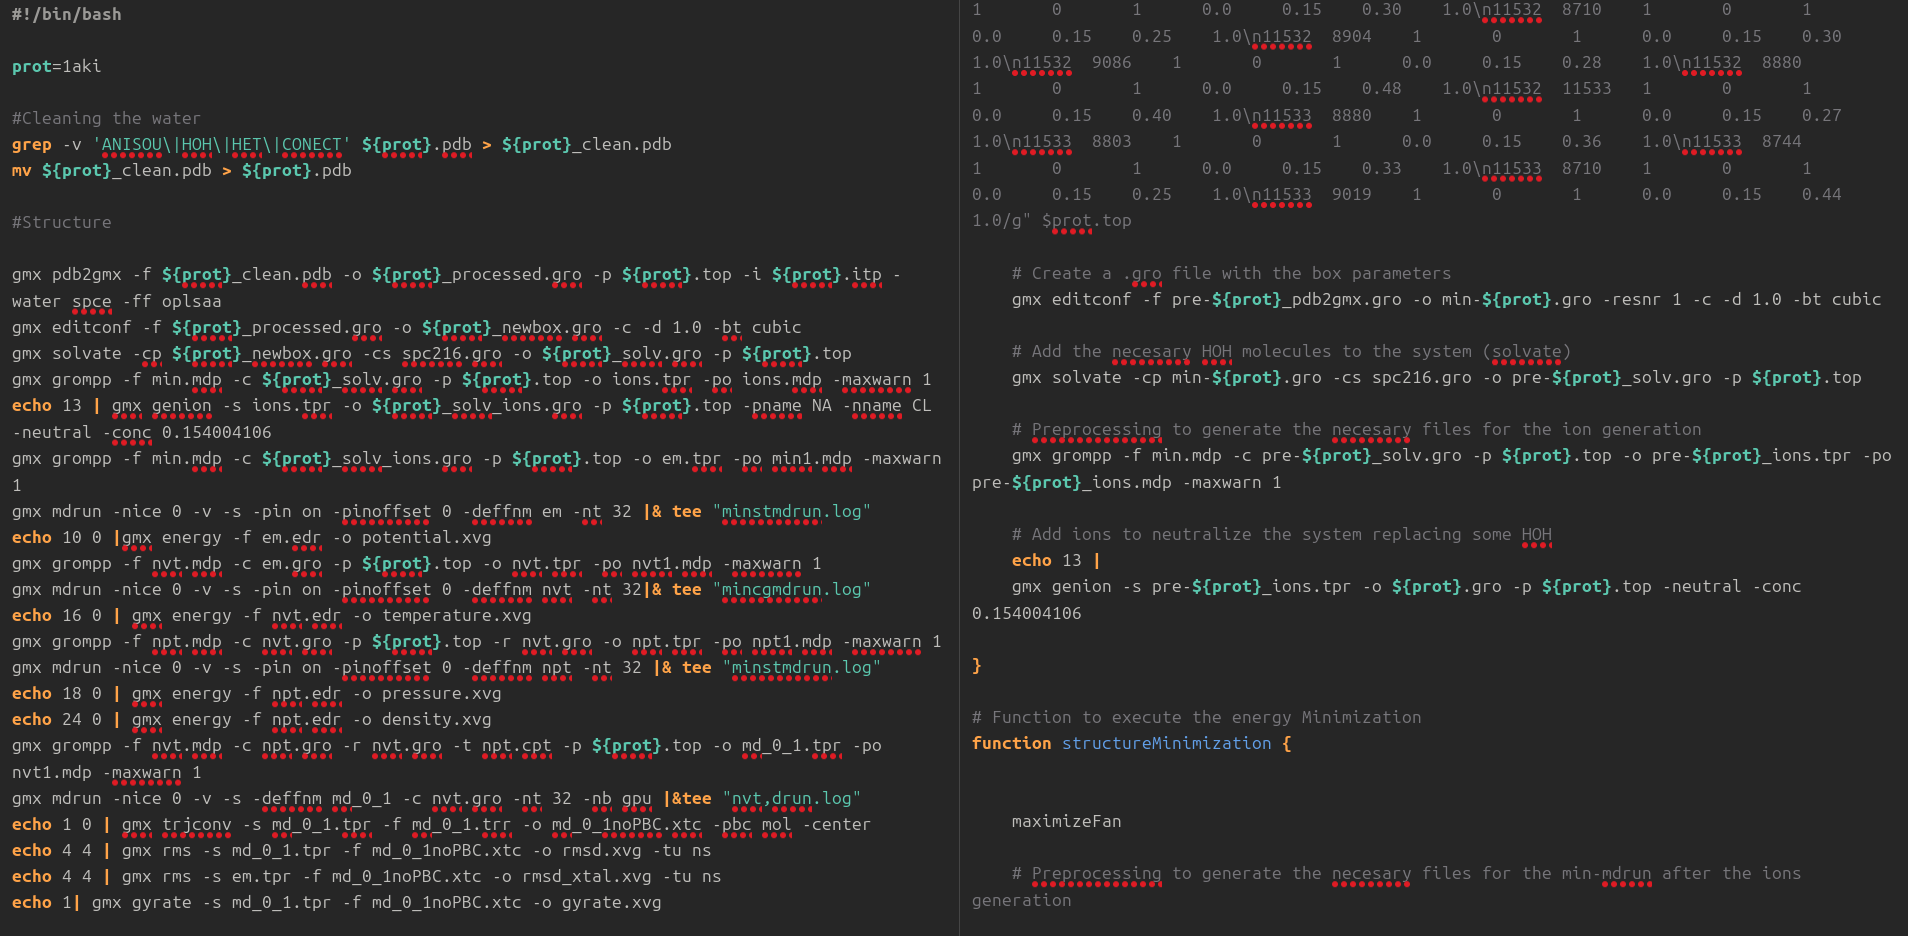
\includegraphics[width=14cm]{img/scrip.png}
            \caption{Aplicación de lenguaje Bash}
            \label{Fig:BashScript}
        \end{figure}
        
           
        \subsubsection{Conclusiones y recomendaciones}
        Concluimos en que el desarrollo de la ingeniería en bioinformática es un camino que requiere de muchos saberes previos debido a la complejidad que se tiene en el desarrollo, gestión y análisis de la data, dentro de la carrera de Ingeniería Biotecnológica, a la cual pertenezco, se evaluó la importancia de la bioinformática centrado al análisis de secuencias como son los alineamientos, incluyendo la búsqueda de soluciones a la transcriptómica, pero se recomienda ampliar el campo de visión para lo que es loa comprensión de los diversos softwares y posiblemente el desarrollo de una nueva optimización de data genómica podría salir a relucir de parte de un ingeniero biotecnólogo.

    \subsection{Actividad 2: Inducción a la Dinámica Molecular}

         \subsubsection{Objetivos} 
            \begin{enumerate}
                \item Aplicar los saberes previos de lectura Bash para interpretar los comandos en Gromacs.
                \item Comprender la aplicación de los campos de fuerza usados en Gromacs.
                \item Analizar los datos resultantes en el ámbito biológico y fisicoquímico.
            \end{enumerate}

         \subsubsection{Justificación}
         Para una persona que está inspirada en el descubrimiento del funcionamiento de estructuras como lo son las estructuras y maquinarias moleculares de la célula es necesario comprender que existe ciencia detrás del análisis de data de las secuencias y estructuras 3D encontradas en bases de datos como lo es PDB, NCBI, UnitProt, entre otras. Esta ciencia de manipulación de data se basa en el retorno de la estructura a su estado fisiológico.
         
         Pero ¿Por qué transformar una estructura al estado fisiológico? Es algo que también me pregunté, ¿no se supone que la data encontrada ya está lista para usarse?, pues la respuesta corta es "no". La data encontrada en las bases de datos son aproximaciones o en forma mas sencilla de explicar, es una simple foto de un cristal. Dentro de un cristal todo es compacto es decir las moléculas están totalmente compactadas y es asi como se encuentran en las estructuras 3D que normalmente vemos y es nuestro deber pasarlas a un estado estable fisiológico que es como comúnmente encontramos a las proteínas en nuestro organismo.
         
         Para ello usamos las herramientas propuestas por un software llamado Gromacs que a traves de diversos comandos nos brinda la ayuda para pasar de una molécula compactada a una molécula a la que se le puede captar en una vibración fisiológica ayudándonos a contemplar las características fisicoquímica que presenta estando se encuentra estable.

         \subsubsection{Metodología}
         
         \subsubsection{Resultados y discusión}
         Gromacs es un software complejo que nos ayuda a poder encontrar la estabilidad fisiológica de las moléculas y encontrar las características de la dinámica molecular de una proteína y es elegido por muchos por la gran variedad de herramientas que nos ofrece como lo es correr dinámicas moleculares con ligando o mantener encontrar interacciones de dominios transmembranales transmembranales, pero por el momento podemos afirmar que se comprendió el funcionamiento de la herramienta de dinámica molecular.
         \subsubsection{Evidencias}

         \subsubsection{Conclusiones y recomendaciones}  

    \subsection{Actividad 3: Planteamiento de un proyecto de Investigación}

         \subsubsection{Objetivos} 
         \subsubsection{Justificación}
         \subsubsection{Metodología}
         \subsubsection{Resultados y discusión}
         \subsubsection{Evidencias}
         \subsubsection{Conclusiones y recomendaciones} 

    \subsection{Actividad 4: Asistencia de investigación para estudiantes de intercambio}

         \subsubsection{Objetivos} 
         \subsubsection{Justificación}
         \subsubsection{Metodología}
         \subsubsection{Resultados y discusión}
         \subsubsection{Evidencias}
         \subsubsection{Conclusiones y recomendaciones}
    


    
      
        
\section{Discusión}
    

En el campo de la biotecnología podemos encontrar varias ramas en diferentes disciplinas como la Biotecnología ambiental, industrial, entre otras. Una de las disciplinas actuales que es muy requerida por la facilidad que tiene en internarse dentro de experimentos de alta complejidad, la compresión de sistemas celulares completos, la bioquímica de las proteínas, la regulación de la expresión de genes, asi como la ayuda en la optimización de terapias contra diferentes patologías, es la bioinformática.

Existe muchas discusiones sobre el tema de la derivación de la bioinformática a partir de la biología computacional, o por lo contrario se afirma de una gran diferencia entre ambas disciplinas.
Personalmente, mi opinion es que la bioinformática es muy requerida por la gran comprensión que puede darnos a conocer a partir del análisis de datos informáticos y par ello se requiere la comprensión del sistema completo celular y para que eso pueda suceder es necesario el conocimiento de la biología computacional que nos aporta las herramientas para simular las estructuras celulares con la alta complejidad fisicoquímica y matemática que tiene cada estructura proteica y sus diferentes alteraciones o interacciones.
   
Son estas inquietudes que demuestran que un internamiento a la bioinformática debe empezar por una comprensión completa de las interacciones y comportamientos de diferentes genes del organismo, es decir, la parte de la biología computacional o como otras personas lo llaman "la parte teórica" que abarca la proteómica, transcriptómica, metabolómica, entre otras disciplinas adscritas al grupo de las "-omicas" y por ende interesadas en dilucidar los comportamientos moleculares. 
   
Dentro de la Universidad Católica de Santa María existe un centro especializado en la comprensión de diferentes estructuras celulares como lo es el Centro de Investigación en Ingeniería Molecular (CIIM) a cargo del doctor "Badhin Gomez Valdez" renombrado ponente especializado en química computacional que se encargó de investigar las interacciones y comportamientos de diferentes estructuras proteicas con diversos ligandos, proteínas o comprender las patologías desde un punto de vista informático.
   
Es allí donde se inició la aventura de mis prácticas pre-profesionales con el objetivo expreso de aprender todo lo necesario para comprender la fisiología celular iniciando con un adiestramiento informático, pasando por un proceso de comprensión y análisis bibliográfico y culminando con la comprensión del uso de diferentes herramientas como lo es el alineamiento de secuencias, interacciones proteína-proteína, proteína-ligando para culminar con un entendimiento cuántico completo sobre los comportamientos que pueden tener diferentes proteínas a cambios dentro de su entorno ya sea por un fármaco proteína o alteraciones en su via de señalización.
   
El objetivo de este informe es narrar las actividades realizadas y logros encontrados en estas primeras 5 semanas como practicante pre-profesional en el Centro de Investigación en Ingeniería Molecular (CIIM).


\section{Evidencias}
En esta sección, se adjuntan documentos y evidencias relevantes que respalden las actividades y logros mencionados en la sección anterior. Esto puede incluir informes técnicos, presentaciones, fotografías, resultados de experimentos, tablas, gráficas, entre otros.

\section{Conclusiones y Recomendaciones}


%%%%%%%%%%%%%%%%%%%%%%%%%%%%%%%%%%%%%%%%%%%%%%%%%%%%%%%%%%%%%%%%%%%%%%%%%
%%%%%%%%%%%%%%%%%%% Agrega cronograma si nos piden %%%%%%%%%%%%%%%%%%%%%%%
%%%%%%%%%%%%%%%%%%%%%%%%%%%%%%%%%%%%%%%%%%%%%%%%%%%%%%%%%%%%%%%%%%%%%%%%%


\section{Bibliografía}


\bibliography{Bibliografia.bib} % Reemplaza "bibliografía" por el nombre de tu archivo .bib


\section{Anexos}
Agregue algunos anexos de ser necesario.



\end{document}